\documentclass{article}

%package setup
\usepackage{graphicx}
\usepackage{amsmath}
\usepackage{fancyhdr}
\usepackage[margin=1in]{geometry}
\usepackage{comment}
\usepackage{placeins}
\usepackage{parskip}
\usepackage{subcaption}
\usepackage{appendix}
\usepackage{soul}
\usepackage{comment}
\usepackage[hidelinks]{hyperref}
\usepackage{matlab-prettifier}
\usepackage{minted}
\usepackage{enumitem}
\usepackage{float}
\usepackage{textcomp, gensymb}

\pagestyle{fancy}
\fancyhf{} % Clear header/footer settings
\rhead{\thepage} % Page number on the right in the header
\lhead{ASE375 Lab Report 2} % Your lab report title on the left

\begin{document}

\begin{titlepage}
  \centering
  
\includegraphics[width=10cm]{ase-logo-formal.png}  % Adjust the width as needed
  \vspace{1cm}  % Add some vertical space
 
  \Large \textbf{ASE 375 Electromechanical Systems}\\
  \large \textbf{Section 14115}\\
  \vspace{0.5cm}
  \textbf{Monday: 3:00 - 6:00 pm}\\
 
  \vspace{1cm}
 
  \hrule
  \vspace{0.5cm}
 
  \Huge \textbf{Report 2:\\
  Temperature Sensor Measurements}\\
  \Huge \textbf{}\\
 
  \vspace{0.5cm}
  \hrule
 
  \vspace{1cm}
 
  \normalsize \textbf{Andrew Doty, Andres Suniaga, Dennis Hom}\\
  \normalsize \textbf{Due Date: 02/12/2024}
 
\end{titlepage}
\newpage

\tableofcontents
\thispagestyle{empty}
\newpage

\section{Introduction}
This experiment consisted of measuring temperature with three different sensors: a Thermocouple, Thermistor, and an Integrated Circuit Temperature sensor. Data collection was made possible through a Data Acquisition (DAQ) system used to process the different temperature measurements in LabVIEW, a graphical interface that modeled the temperature sensors' measurements in real-time. 

The purpose of this experiment was to learn how to simulate our data through LabVIEW along with observing and understanding the behaviour of the three temperature sensors in different environments: $(1)$ at room temperature, $(2)$ in water near freezing conditions, and $(3)$ in water closer to boiling conditions. 

\section{Equipment}
The equipment used in this experiment include the following:  

K-type Thermocouple:  Temperature sensor with two different metals joined together at one end.  A K-type thermocouple uses Chromel-Alumel metals.  It will be connected to the DAQ via the NI 9211 thermocouple input module.  

SA1-TH Series Thermistor:  Temperature sensor that measures electrical resistance as a response to a change in temperature.  It is connected to the NI 9215 via breadboard in its own circuit with $1\text{k}\Omega$ resistor.
\begin{figure}[H]
    \centering
    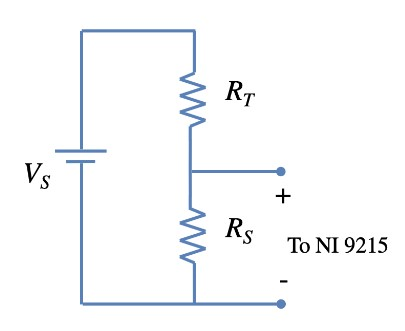
\includegraphics[width=0.25\textwidth]{Lab 2/lab2images/thermistor_circuit.jpg}
    \caption{Thermistor Circuit}
\end{figure}

TMP36 Temperature Sensor: Analog low voltage sensor.  It is connected to the NI 9215 via the breadboard.  

Breadboard: a reusable solderless prototyping board used for building electronic circuits. Components are inserted into interconnected rows and columns of holes, allowing for easy and temporary assembly of circuits for testing and experimentation.

Circuit Components:  various length male-to-male jumper wires, $1\text{k}\Omega$ resistor, 5V power supply.

DAQ:  Data Aquisition system that digitizes analog information into "bins" for a computer.  The specific DAQ had two units, the NI 9215 and NI 9211.  Specific Datasheets for each are included in the appendices.  

Thermometer:  Regular mercury thermometer, using change in volume as a response to a change in temperature.  Used to measure true temperature with 0.5 degrees least count.  

Water:  Access to water at two temperatures, near boiling, and ice cold. 

\section{Procedure}
\begin{figure}[H]
\centering
\includegraphics[width=0.5\textwidth, angle = -90]{lab2images/circuit_board_mug_and_sensors.jpg}
\caption{Temperature Sensors, Water mug, and Breadboard circuit}
\end{figure}

The first step was to setup LabVIEW to simulate the temperature sensors. Before the lab session, the DAQ was connected to the computer and various sensors were connected to the DAQ in modules NI 9211 and NI 9215. The following simulation was created by creating a virtual DAQ by rightclicking the desktop and searching for a DAQ in the popup menu. Next we created a collector and set the value to 500000, indicating we were taking 500000 samples. We imported a split signal and ran the output from the collector into the split signal. Each of the signals went to a specific graph, one for each sensor. A structure in LabVIEW (while loop) enclosed the system and was set to run for the number of iterations specified in the collector. And a "Write to Measure File" block was placed outside of the while loop to save the data to a file. We right-clicked the block and selected "Excel File" and set the file name to not overwrite.

Now that our digital sensing was set up, we had to create the physical circuits. The thermistor was connected to the NI 9215 module, and the TMP36 was connected to the same module. The thermocouple was connected to the NI 9211 module. The thermistor was connected to a $1\text{k}\Omega$ resistor in a voltage divider configuration. The TMP36 was connected to the 5V power supply and the NI 9215 module. The thermocouple was connected to the NI 9211 module. This breadboard configuration is shown in the figure above.

\subsection{Part 1} % Subsection 1

To gather the room temperature data, we placed the sensors in an unused area in the lab room and let them sit for a few minutes without any of us moving near them or touching them, to stop heat from diffusing through the rubber casing of the wire or through the air. We then ran the LabVIEW simulation for 1 minute and saved the data to an Excel file with a frequency of at least 100 hertz. The results of the simulation are shown in the figures below.

\subsection{Part 2} % Subsection 2

\subsubsection{Part 2a: Hot Water} % Subsubsection 1

We used the electric kettle in the lab to heat up water to near boiling. We then started the LabVIEW simulation, waited a couple seconds to make sure the results were normalized, and suddenly placed the sensors in the water. After letting them sit for a few minutes to reach equilibrium, we saved the data to an Excel file with a frequency of at least 100 hertz. The results of the simulation will also be shown in the results section below.

\subsubsection{Part 2b: Water Cooling} % Subsubsection 2

Using the same simulation from last time, we timed from when the water was at its hottest temperature until the water went to \(60^\circ\) C, as that is considered the cold end of the ideal coffee drinking temperature, which is less than the overall temperature. However, after checking the EPA's recommendations, they listed \(40^\circ C\) as the optimal high-end temperature for drinking water. We placed markers at each of these temperatures to be safe and saved the data to an Excel file with a frequency of at least 100 hertz. The results of the simulation will also be shown in the results section below.

\subsubsection{Part 2c: Ice-Hot} % Subsubsection 3

To give us more information to calibrate our sensors, we took a bowl of water with \( 2^\circ \) C temperature and a bowl of water with \( 90^\circ \) C temperature. We placed the sensors in the cold water, took a measurement, and waited around 1 minute for the sensors to each equilibirum. We then quickly placed the sensors in the hot water while taking a measurement to check how long it takes for the sensors to reach steady state, and what the time constant was.

\subsubsection{Part 2d: Quick Changes} % Subsubsection 4

Lastly, after the sensor had reached steady state in the water above, we took the sensors out of the water while taking a measurement to see how quickly the sensors would return to room temperature. We saved the data to an Excel file with a frequency of at least 100 hertz. The results of the simulation will also be shown in the results section below.

\subsubsection{Part 2e: Sensor Repetition} % Subsubsection 5

We repeated the above steps for each sensor to see if there were any differences in the sensors' responses to the different temperatures. The results of the simulation will also be shown in the results section below.

\section{Data Processing}
\subsubsection*{Variables}
\begin{enumerate}[label = \roman*.]
    \item \(N = \) Number of Samples
    \item \(f_{s} = \) Sampling Frequency, $s^{-1}$
    \item \(\Delta t_{s} = \) Sampling Interval, $s$
    \item \(\gamma = \) Confidence Level, \%
    \item \(R_{S} = \) Sensor Resistance, Ohms = $\Omega$ (In this experiment it will be $1\text{k}\Omega$)
    \item \(V_{S} = \) Source voltage, Volts = $V$ ($5\;V$ for this experiment)
    \item \(R_{T} = \) Themistor resistance, $\Omega$
\end{enumerate}

\subsubsection*{Equations}
\begin{enumerate}[label = \Roman*.]
    \item Sample Mean: \(\bar{x} = \dfrac{1}{N}\displaystyle\sum_{i=1}^{N} x_{i}\) 
    \item Standard Deviation of finite $N$, normalized by $N-1$: \(S_{x} = \sqrt{\displaystyle\sum_{i=1}^{N} \dfrac{(x_{i} - \bar{x})^{2}}{N-1}}\)
    \item Standard Deviation of the Mean: \(\dfrac{S_{x}}{\sqrt{N}}\)
    \item Average Measurement w/ Confidence Interval: \(\bar{x} \pm t_{stat}\cdot \dfrac{S_{x}}{\sqrt{N}}\)
    \item \textit{Steinhart-Hart Relation}: \(\dfrac{1}{T} = A + B\cdot ln(R_{T}) + C\cdot (ln(R_{T}))^{3}\), where $A$, $B$, $C$ are the Thermistor's calibration coefficients.
\end{enumerate}
 
\begin{figure}[H]
\centering
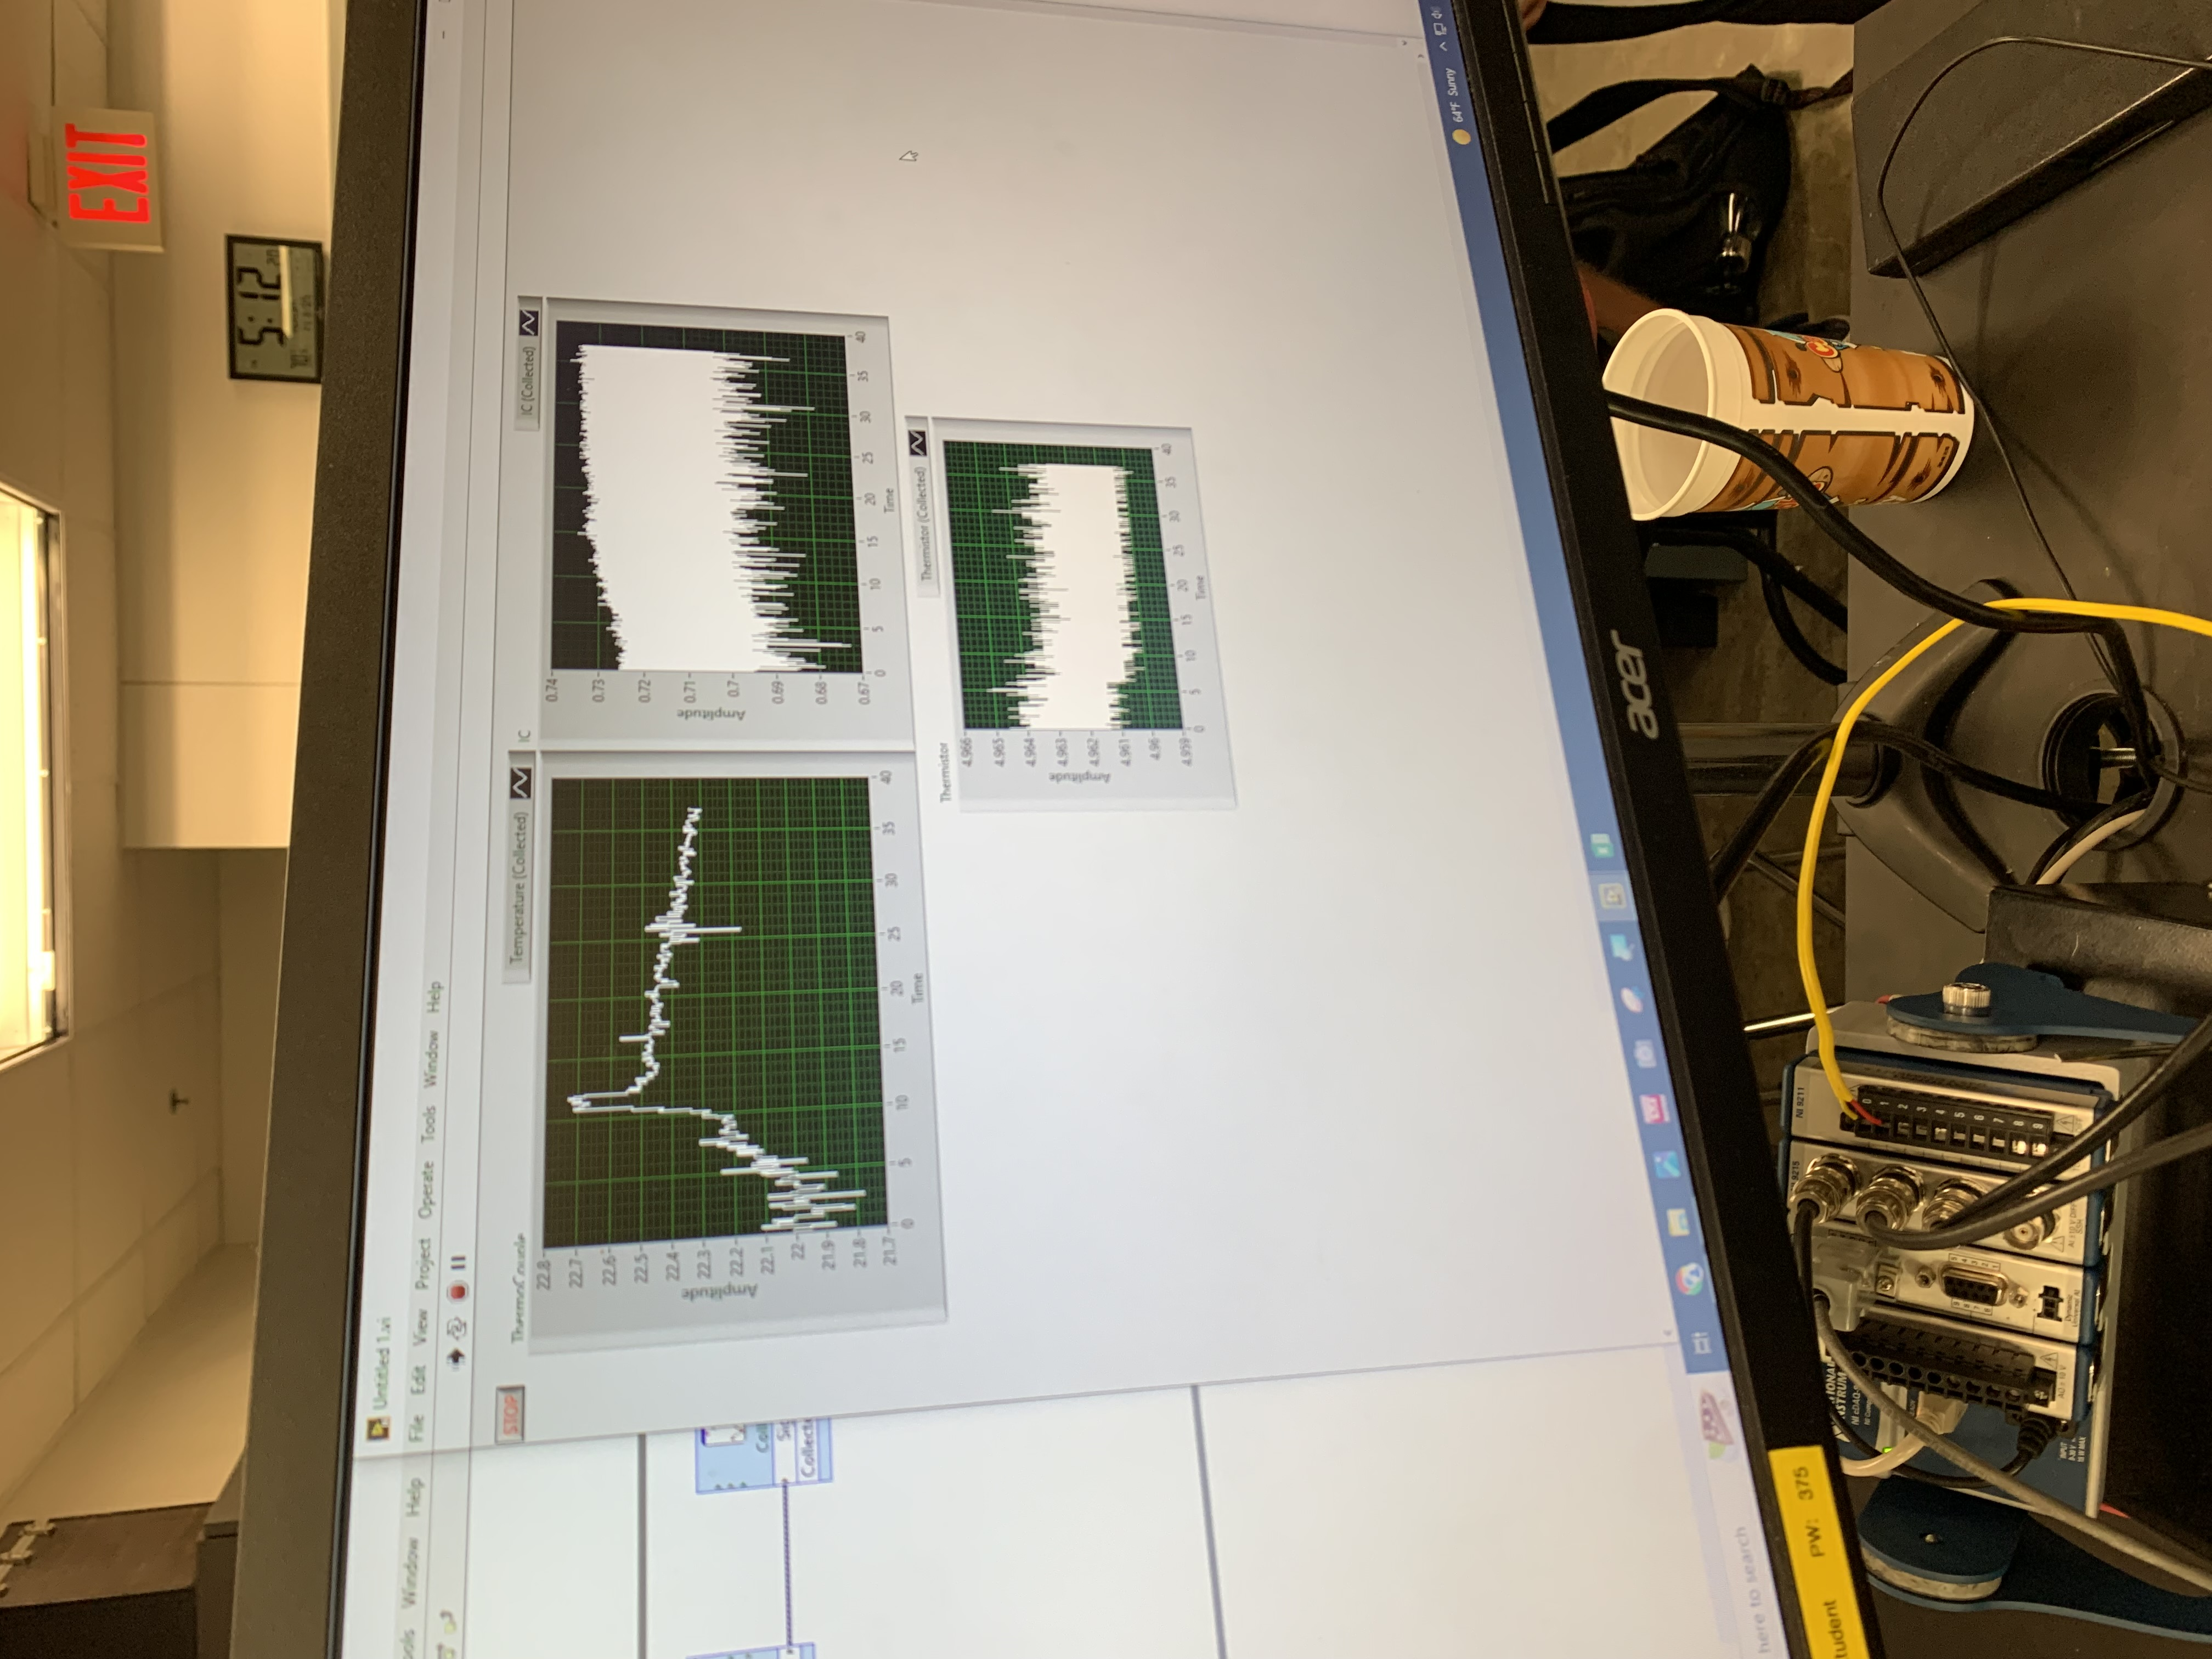
\includegraphics[width=0.5\textwidth, angle = -90]{lab2images/labview_plots.jpg}
\caption{Plotting data on LabVIEW}
\end{figure}

\subsection{Part 1: Ambient Temperature}
In Part 1 of the experiment we take measurements of the laboratory room temperature using each of the three sensors: thermocouple, thermistor, and IC TMP36. The data displayed below shows the temperature sensors at work for $1$ minute of sampling at $f_{s} = 1000\; s^{-1}$. This means $\Delta t_{s} = (f_{s}\cdot 60)^{-1} = 1.6667\times10^{-5}\; \text{minutes}$.

\begin{figure}[H]
    \centering
    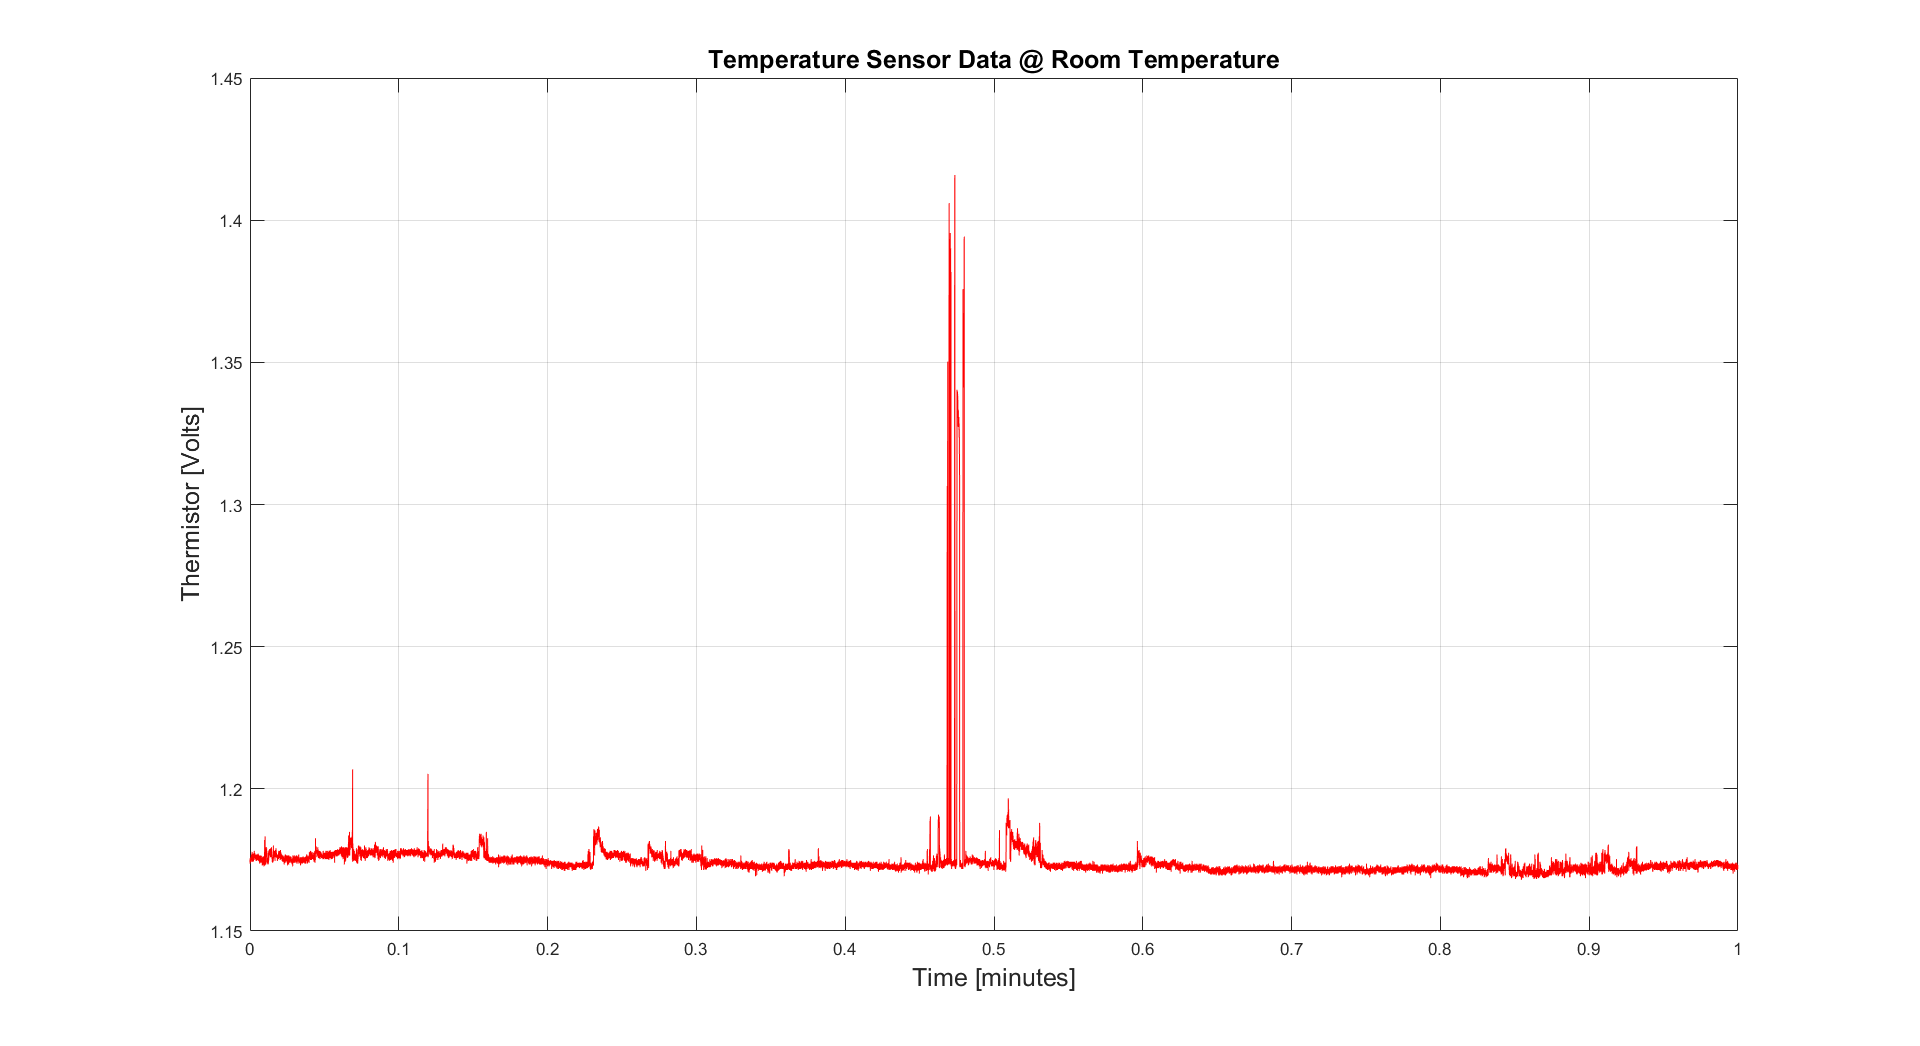
\includegraphics[width=0.655\textwidth]{lab2images/thermistor_volt_roomtemp_1min_plot.png}
    \caption{Thermistor at ambient temperature}
\end{figure}

\begin{figure}[H]
    \centering
    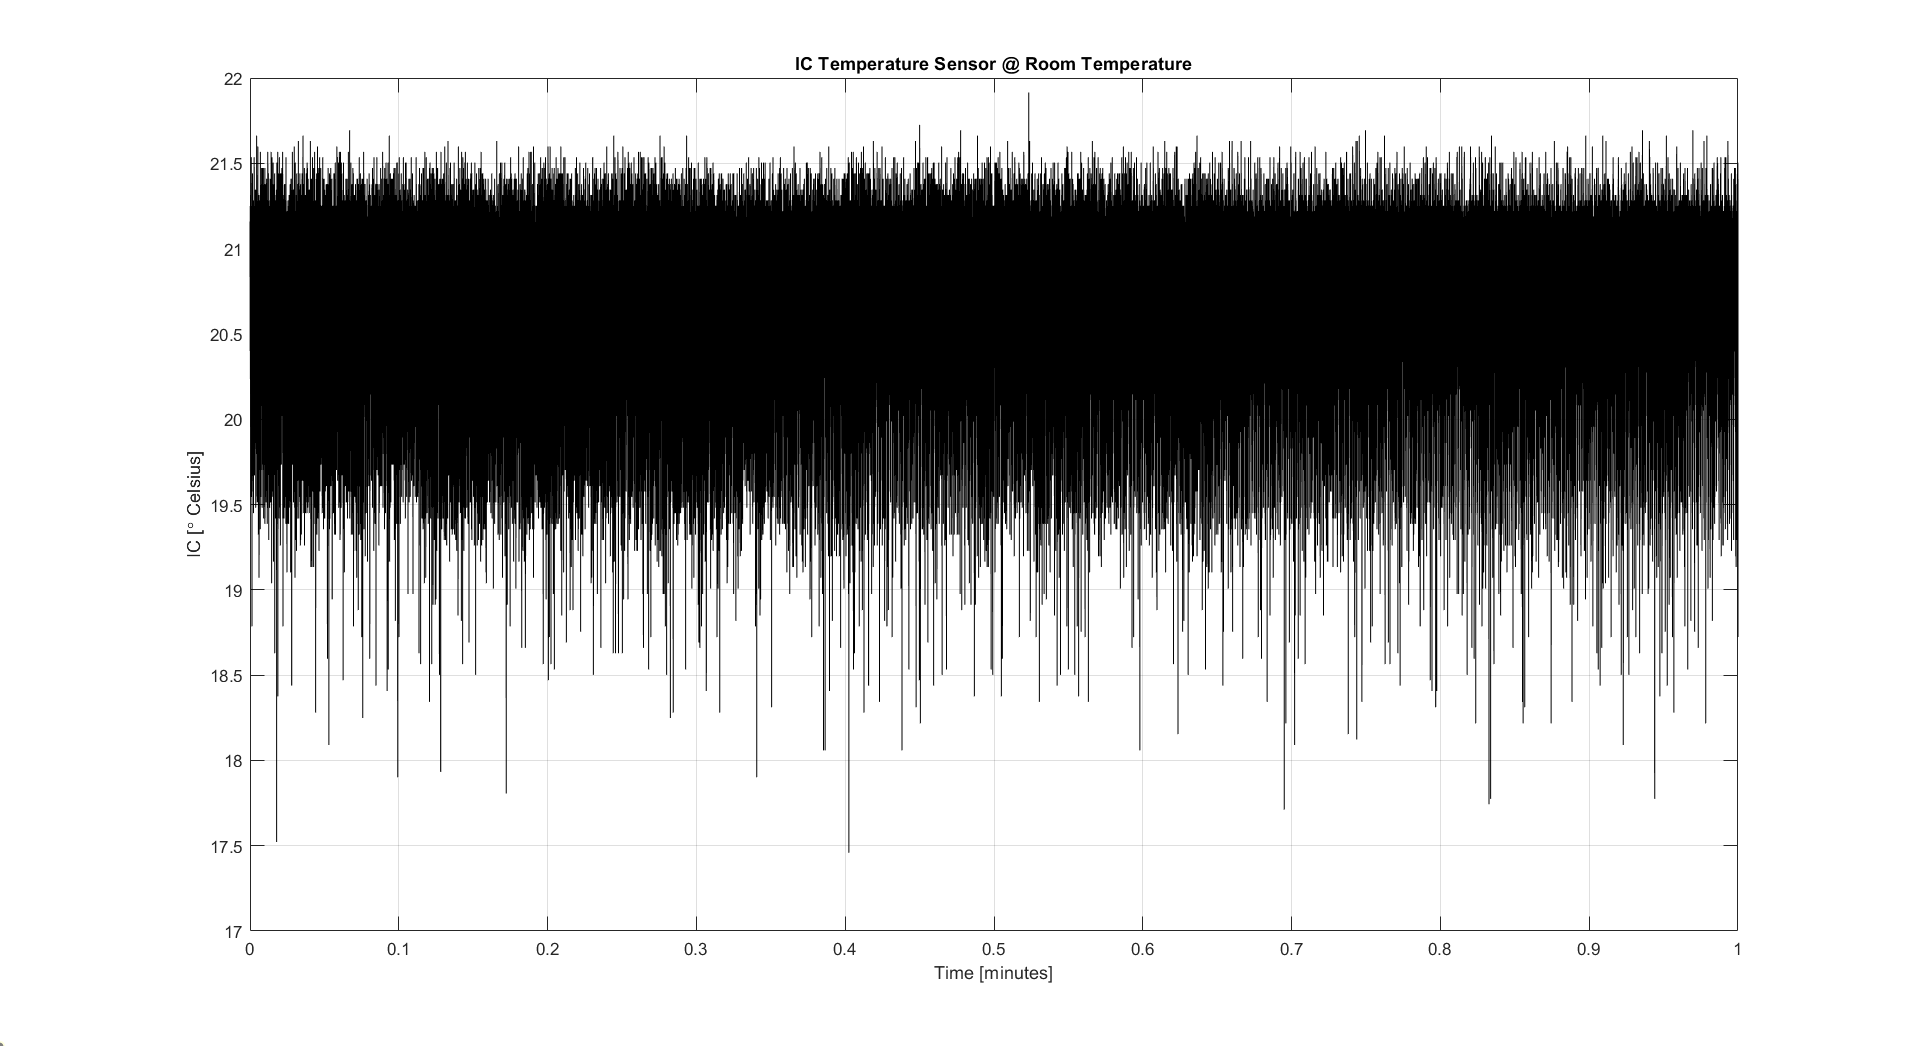
\includegraphics[width=0.655\textwidth]{lab2images/ICTMP36_roomtemp_1min_plot.png}
    \caption{IC TMP36 at ambient temperature}
\end{figure}

\begin{figure}[H]
    \centering
    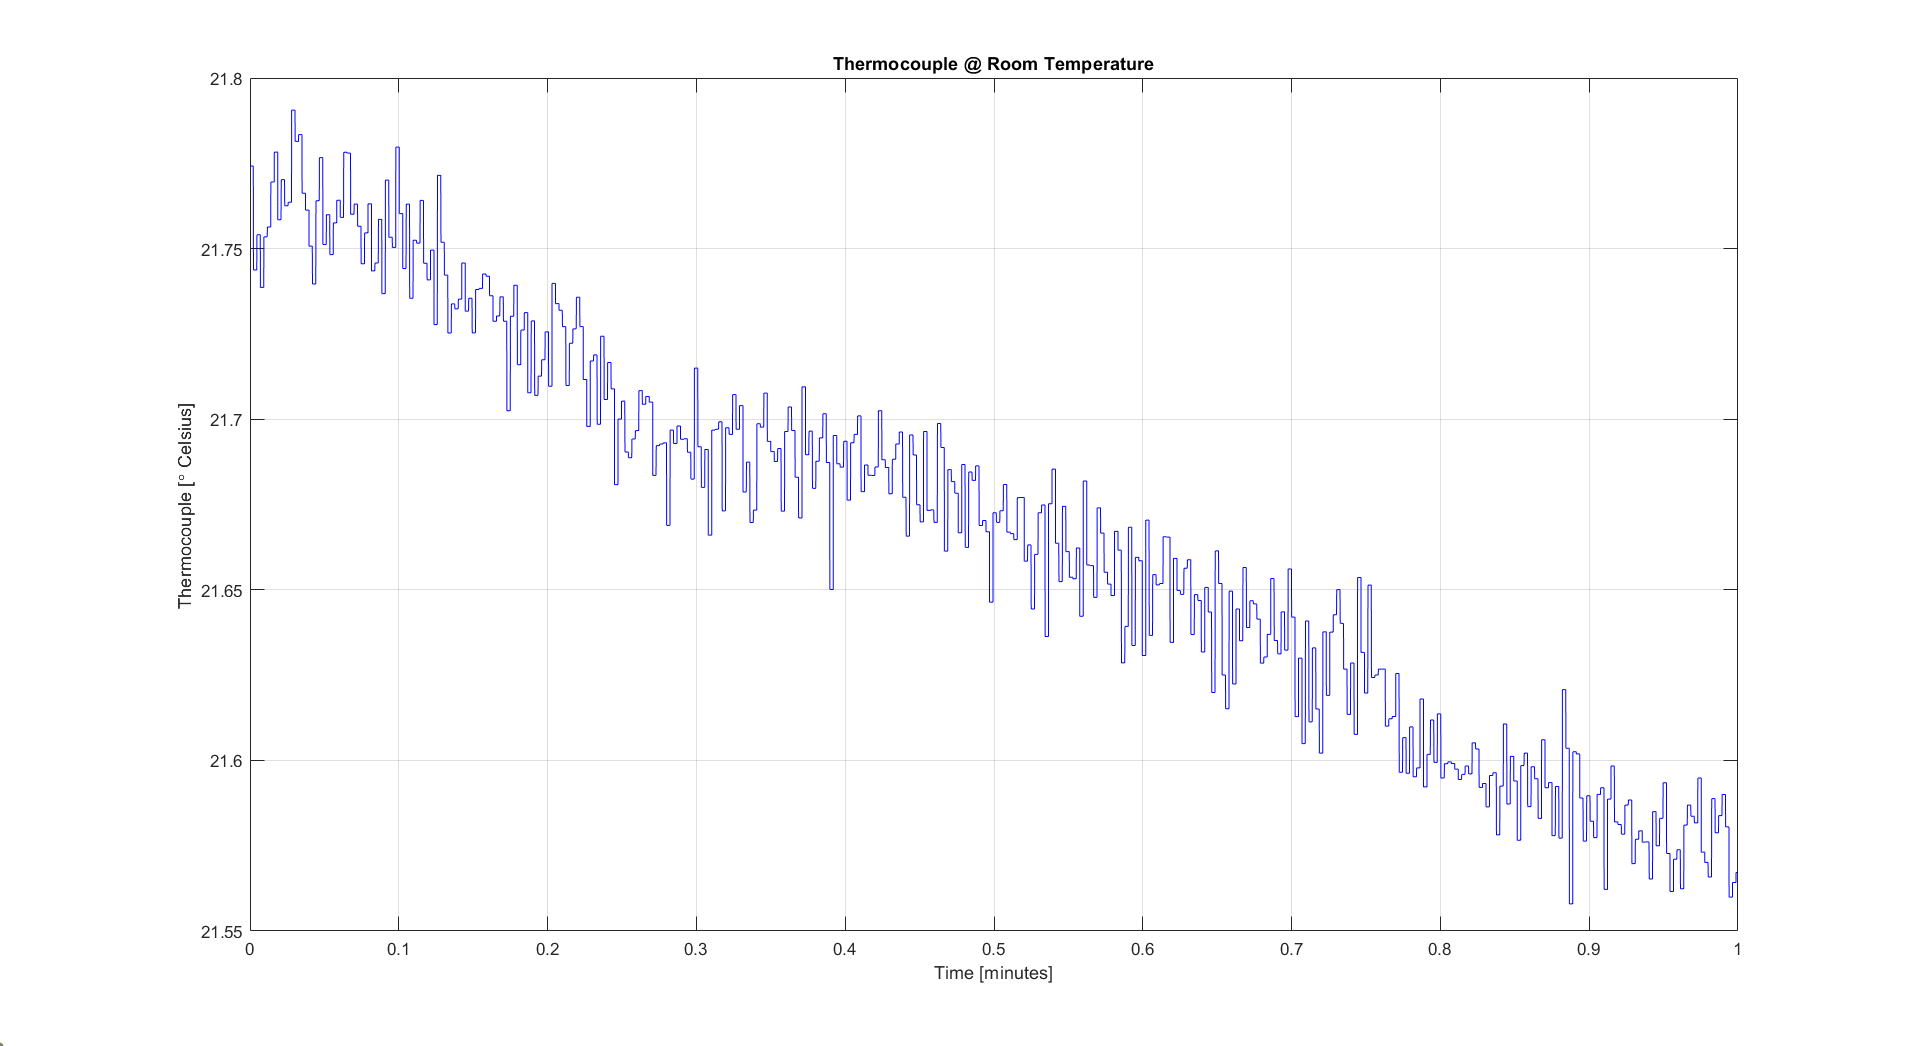
\includegraphics[width=0.655\textwidth]{lab2images/thermocouple_roomtemp_1min_plot.png}
    \caption{Thermocouple at ambient temperature}
\end{figure}

There are small spikes occurring around half of the period for the Thermistor's output. This disturbance could have been due to the Thermistor's sensitivity to very small changes in temperature, possibly due to slight movement (increased kinetic energy correlates to increased thermal energy).

The TMP36 data appears to be white noise for the entirety of the $1$ minute period with a large temperature interval. This shows the inaccuracy of the TMP36 when comparing to the other two sensors.

Similar to the small change in the Thermistor's output, the Thermocouple sees small changes as it is decreasing to a steady-state.  

The IC/TMP36 sensor originally outputs voltage. This was converted to $\degree C$ by taking the IC TMP36 output, say $x_{V}$ ($V$ for volt), and converting by $x_{\degree C} = 100\cdot(x_{V}-0.5)$. This conversion comes from the TMP36 datasheet ($10\,mV/\degree C$ w/ $500\,mV$ offset):
\begin{center}
    \href{https://www.analog.com/media/en/technical-documentation/data-sheets/tmp35_36_37.pdf}{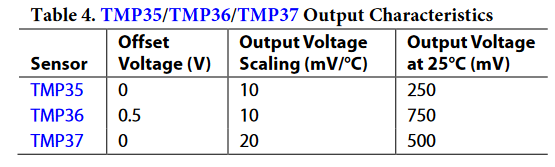
\includegraphics[width = 0.6\textwidth]{lab2images/tmp36_offset_documentation.png}}
\end{center}



\subsubsection{Mean Temperature in Laboratory w/ Confidence Interval}
Calculation of the mean temperature with confidence interval of $\gamma = 95\%$ was implemented through MATLAB as shown below:
\begin{lstlisting}[style=Matlab-editor]
% Confidence Interval in Laboratory
gamma = 0.95; %95 percent confidence

Fz = 0.5*(1+gamma);

nu = Q-1; %DOF

p = (1-gamma)/2; %probability

tstat = tinv(p,nu); 

% (SAMPLE MEANS) Mean w/ Confidence Interval
avg_unc_thermistor = [mean(thermistordata) 
                     tstat*std(thermistordata)/sqrt(Q)];

avg_unc_IC = [mean(ICdata) 
             tstat*std(ICdata)/sqrt(Q)];

avg_unc_thermocouple = [mean(thermocoupledata)  
                       tstat*std(thermocoupledata)/sqrt(Q)];
\end{lstlisting}

We define $F(z) = \frac{1}{2}(1+\gamma) = 0.9750$. The degrees of freedom (D.O.F.) $\nu = N - 1 = 59,999$ where $N=60,000$ samples. Set $P=\dfrac{1-\gamma}{2}=0.0250$. Using MATLAB function \textit{tinv}, we calculate the t-statistic to be $t_{stat} = -1.960$ or according to the \hyperlink{1}{t-distribution tables} this is also just $t_{stat}=1.960$.

Below are the average temperatures w/ the confidence interval for each of the three sensors:
\begin{itemize}
    \item Thermistor: \(1.1743 \pm 0.0001\; V \)
    \item IC/TMP36: \(20.8415 \pm 0.0038\; \degree C\)
    \item Thermocouple: \(21.6671 \pm 0.0005\; \degree C\)
\end{itemize}


\subsection{Part 2: Hot and Cold Water}


\section{Results and Analysis}
(Answer Observation Questions from Part 2)


\section{Conclusion}




\newpage
\thispagestyle{empty}  % Clear header/footer
\begin{center}
	\vspace*{\fill}
	{\Huge Appendices}
	\vspace*{\fill}
\end{center}

% Start appendices
\newpage
\begin{appendices}
\pagestyle{fancy}
\renewcommand{\thefigure}{A\arabic{figure}}
\setcounter{figure}{0}

\section*{Appendix: t-Distribution Tables}
\hypertarget{1}{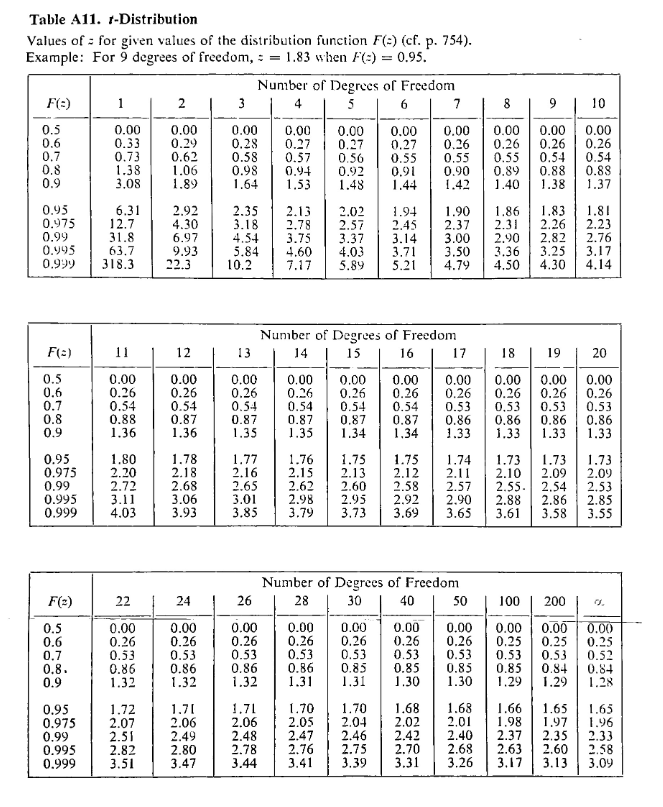
\includegraphics[width=0.95\textwidth]{Lab 1/t_distribution_Table_lecture3.png}}
\end{appendices}

\end{document}
